\chapter{Struttura e progettazione}
\label{cap:struttura-progettazione}

\intro{In questo capitolo viene presentata la struttura principale del progetto
      e le attività di progettazione del servizio. Vengono inoltre descritte le
      tecnologie utilizzate durante lo sviluppo e le scelte architetturali.}\\

\section{Tecnologie utilizzate}

Di seguito vengono elencate e descritte le tecnologie utilizzate durante lo sviluppo del
progetto di stage.

\subsection{Back-end}

\subsubsection*{Go}

Go è un linguaggio di programmazione \emph{open source} sviluppato da
\emph{Google} nel 2007. È un linguaggio compilato, staticamente tipizzato e
fortemente tipizzato, con una sintassi simile a quella del linguaggio \emph{C}.
Il linguaggio è stato progettato per semplificare la programmazione di sistemi
distribuiti, con particolare attenzione alla concorrenza e alla
comunicazione in rete. \\
È un linguaggio che segue una filosofia di scrittura del codice molto semplice e
nel mio progetto ho seguito alcune delle linee guida proposte dalla comunità di
sviluppatori, come ad esempio la struttura del codice e la gestione degli errori
con il \emph{pattern} \emph{error handling}. \\
Per il mio progetto ho utilizzato la versione 1.21 di \emph{Go}, al fine di
utilizzare l'ultima versione attualmente disponibile.\\
Una caratteristica particolare di \emph{Go}, che verrà mostrata successivamente
nella sezione dedicata alla codifica, è la capacità di rendere pubbliche le
funzioni o le variabili semplicemente scrivendo il nome con la lettera iniziale
maiuscola: questo sistema permette di identificare a colpo d'occhio le funzioni
o le variabili pubbliche, mantenendo il codice semplice da leggere e scrivere. \cite{go}

\subsubsection*{AWS CDK}

\emph{AWS Cloud Development Kit} (AWS CDK) è un \emph{framework} di sviluppo
\emph{open-source} che permette di definire le risorse \emph{AWS} utilizzando
uno o più linguaggi di programmazione. Questo \emph{framework} prevede il pieno
supporto al linguaggio di programmazione \emph{Go}. \\
Nel progetto è stato utilizzato per definire lo \emph{stack} contenente le risorse \emph{AWS}
necessarie al funzionamento del servizio, come la funzione \emph{Lambda}, le
tabelle \emph{DynamoDB} e i \emph{bucket S3}. \cite{go-aws-cdk}

\subsubsection*{AWS SDK}

\emph{AWS Software Developement Kit} (AWS SDK) è un insieme di librerie che
permettono di interagire con i servizi \emph{AWS} utilizzando diversi linguaggi
di programmazione. L'\emph{SDK} prevede il pieno supporto al linguaggio di
programmazione \emph{Go}. \\
Nel progetto è stato utilizzato per interagire con le risorse \emph{AWS}
definite con \emph{AWS CDK}. \cite{go-aws-sdk}

\subsubsection*{AWS Lambda}

\emph{AWS Lambda} è un servizio \emph{serverless} che permette di eseguire del
codice senza dover gestire l'infrastruttura sottostante. Il servizio permette di
eseguire del codice in risposta a determinati eventi, come ad esempio una
richiesta \emph{HTTP} o un inserimento di dati in una tabella \emph{DynamoDB}.
\\
Nel progetto è stato utilizzato per eseguire il codice che permette di
di effettuare la conversione delle immagini desiderate, recuperando una
configurazione da una tabella \emph{DynamoDB}, recuperando l'immagine da
convertire da un \emph{bucket S3} e salvando il risultato in un secondo
\emph{bucket S3}, dopo aver salvato le informazioni legate alla conversione in
una seconda tabella \emph{DynamoDB}.

\subsubsection*{AWS DynamoDB}

\emph{AWS DynamoDB} è un database \emph{NoSQL} completamente gestito, che
supporta strutture di dati di tipo documento e di tipo chiave-valore. Questo
database supporta lettura e scrittura di dati senza degradamento delle
performance generali del servizio. \\
Nel progetto è stato utilizzato per salvare le informazioni legate alle
conversioni effettuate, come ad esempio il nome dell'immagine convertita, il
tipo di conversione effettuata e il momento in cui è stata effettuata la
conversione. È stato inoltre utilizzato per salvare le configurazioni di
conversione, come ad esempio il formato di output e la qualità dell'immagine
convertita.

\subsubsection*{AWS S3}

\emph{AWS S3} è un servizio di \emph{storage} completamente gestito, che
permette di salvare e recuperare dati da una posizione di memoria detta
\emph{bucekt}. Supporta operazioni di lettura e scrittura di dati da parte di
altri servizi, ma può essere utilizzato per gestire \emph{backup} o per servire
siti \emph{web} statici. \\
Nel mio progetto è stato utilizzato per salvare le immagini da convertire e le
immagini convertite.

\subsubsection*{AWS CloudWatch}

\emph{AWS CloudWatch} è un servizio di monitoraggio e gestione delle risorse
\emph{AWS} e delle applicazioni eseguite su \emph{AWS}. Il servizio permette di
raccogliere e monitorare dati di interesse, visualizzandoli in modo sintetico e
intuitivo. \\
Nel progetto è stato utilizzato per monitorare le conversioni effettuate e
raccogliere i \emph{log} presenti all'interno del codice eseguito dalla funzione
\emph{Lambda}.

\subsection{Versionamento}

\subsubsection*{Git}

\emph{Git} è un sistema di controllo di versione distribuito, utilizzato per
tenere traccia delle modifiche effettuate al codice sorgente di un progetto
\glsfirstoccur\gls{software}.

\subsubsection*{AWS CodeCommit}

\emph{AWS CodeCommit} è un servizio di controllo di versione completamente
gestito all'interno dell'ecosistema di \emph{AWS}, che permette di ospitare in modo sicuro e scalabile i \emph{repository}
\emph{Git} privati. \\

\subsection{Librerie e applicazioni esterne}

\subsubsection*{Libvips}

\emph{Libvips} è una libreria \emph{open source} per la manipolazione di immagini
sviluppata in \emph{C}. La libreria è stata sviluppata per essere veloce e
utilizzare poca memoria, ed è ampiamente utilizzata da numerose applicazioni
\emph{web} e \emph{desktop}. \\
Nel progetto è stata utilizzata per effettuare la conversione delle immagini
di formato \emph{JPEG, WebP, PNG, SVG, TIFF e GIF} verso i formati \emph{JPEG} e
\emph{PNG}. La libreria permette di applicare all'immagine il profilo colore
desiderato, permette la rotazione automatica di un'immagine seguendo
l'orientamento presente dei \glsfirstoccur\gls{metadati}
\glsfirstoccur\gls{EXIF} e permette di scalare un'immagine seguendo la larghezza
e l'altezza desiderate. \cite{libvips}

\subsubsection*{GhostScript}

\emph{GhostScript} è un interprete per il linguaggio di descrizione dei file
\emph{PostScript} ed \emph{EPS} (\emph{Encapsulated PostScript}).
Questo interprete permette la conversione delle immagini dai formati \emph{PS,
      EPS e AI} ai formati \emph{JPEG} e
\emph{PNG}. \\
Nel progetto viene richiamato direttamente dal codice \emph{Go} per effettuare
la conversione, specificando il formato di output desiderato. \cite{ghostscript}

\subsubsection*{Darktable}

\emph{Darktable} è un'applicazione \emph{open source} per la gestione e la
modifica di immagini \emph{RAW}. Questa applicazione permette di convertire le
immagini \emph{RAW} in immagini nei formati \emph{JPEG} e \emph{PNG}.
L'applicazione presenta anche una interfaccia \glsfirstoccur\gls{CLI} che
permette di effettuare il processo di conversione immagini richiamandola
direttamente dal codice \emph{Go} del progetto.\\
L'applicazione permette di applicare un profilo colore desiderato e di impostare
la qualità dell'immagine convertita tramite un valore che varia da 0 a 100. \cite{darktable}

\subsubsection*{Go-psd}

\emph{Go-psd} è una libreria \emph{open source} sviluppata in \emph{Go} che
permette di leggere e scrivere file \emph{PSD} (\emph{Photoshop Document}),
senza servirsi di \emph{software} esterni. \cite{go-psd}

\subsubsection*{Imagemagick}

\emph{Imagemagick} è un \emph{software} \emph{open source} per la manipolazione
di immagini, che permette di convertire le immagini da un formato all'altro.
Nel progetto è stata utilizzata solo una minima parte del programma, ovvero
solo il comando \emph{identify}, che permette di recuperare i metadati dai file
di formato \emph{EPS, PS e AI}. \cite{imagemagick}

\subsubsection*{Exiftool}

\emph{Exiftool} è un \emph{software} \emph{open source} per la lettura e la
scrittura dei metadati presenti nei file. Nel progetto è stato utilizzato per
recuperare i \emph{metadati} da tutte le immagini analizzate dal servizio, ad
eccezione dei file di formato \emph{EPS, PS e AI}, che vengono gestiti da
\emph{Imagemagick}.\cite{exiftool}

\section{Struttura del sistema}

Il sistema è composto solamente dalla sezione \emph{back-end}, poiché
non è previsto che l'utente interagisca direttamente con il sistema delle
conversioni. \\
Il sistema si occupa di elaborare le richieste di conversione, di gestirle e di
salvare i risultati negli spazi di \emph{storage} dedicati.

\subsection{Ambiente di sviluppo}

È stato predisposto un ambiente di test, detto \emph{sandbox}, che permette di
testare il servizio serverless sviluppato senza intaccare la struttura e le
funzionalità già presenti in produzione. In questo ambiente è possibile
utilizzare tutte le risorse necessarie al servizio.

\subsection{Configurazione dell'ambiente di sviluppo}

Il progetto di stage necessita di cartelle e file per la configurazione
dell'ambiente di sviluppo e per la configurazione del \emph{deploy}. Più nello
specifico, il progetto segue la struttura qui descritta.

\subsubsection*{\emph{Buildspec}}

Il file \emph{buildspec} è un file di configurazione che contiene la definizione
dello \emph{stack} di risorse da generare su \glsfirstoccur\gls{AWS
      Cloudformation}. \\
Dopo aver effettuato tutti i comandi all'interno del file \emph{buildspec},
viene avviato il processo di \emph{deploy} delle risorse \emph{AWS} definite nel
file \emph{infra.go}. Il file \emph{buildspec} è un file di tipo \emph{YAML},
formato dalle seguenti sezioni:
\begin{itemize}
      \item La sezione \emph{env}, dove vengono specificate le variabili
            d'ambiente utilizzate nel progetto;
      \item la sezione \emph{pre-build}, dove vengono specificati i comandi da
            eseguire prima della \emph{build} del progetto;
      \item la sezione \emph{build}, dove viene specificato il comando per il
            \emph{deploy} del progetto.
\end{itemize}

\subsubsection*{\emph{Infra}}

Il file \emph{infra.go}, presente all'interno della cartella \emph{infra}, è un file di configurazione scritto in linguaggio
\emph{Go}, che contiene la definizione dello \emph{stack} di risorse da
generare.\\
Qui sono state definite le seguenti risorse:
\begin{itemize}
      \item due \emph{bucket S3}, uno dove caricare le immagini da convertire,
            detto \emph{input}, l'altro dove caricare le immagini convertite, detto
            \emph{output};
      \item due tabelle \emph{DynamoDB}, una dove salvare le informazioni legate
            alle conversioni effettuate, detta \emph{jobs}, l'altra dove sono salvate le
            configurazioni delle conversioni da effettuare, detta \emph{client-conf};
      \item una funzione \emph{Lambda}, detta \emph{converter}, che esegue il
            codice presente nel file \emph{main.go}, all'interno della cartella
            \emph{cmd}. La funzione \emph{Lambda} invoca un \glsfirstoccur\gls{container}
            \glsfirstoccur\gls{docker} che permette di eseguire il codice legato
            alla conversione.
\end{itemize}

\subsubsection*{Dockerfile}

Il file \emph{Dockerfile} è un file di configurazione che contiene la
definizione di un \emph{container} \emph{Docker}, in cui sono presenti tutte le
dipendenze necessarie al funzionamento del codice. \\
Quando viene invocata la funzione \emph{Lambda}, viene avviato il
\emph{container} \emph{Docker}, al fine di eseguire il codice in un ambiente
isolato, garantendone la funzionalità \emph{serverless}.

\section{Progettazione}

\subsection{Architettura}

L'architettura del sistema è sviluppata pensando alle \emph{best practices} per
lo sviluppo di servizi \emph{serverless}: in particolare mi sono dedicato alla
scrittura della \emph{business logic} del servizio e delle risorse necessarie al
suo funzionamento. \\
Il sistema prevede l'utilizzo di tre tipi di risorsa \emph{AWS}:
\begin{itemize}
      \item \textbf{\emph{Lambda:}} è la funzione che si occupa di eseguire la
            \emph{business logic} del codice e di inviare e ricevere i dati dalle altre risorse
            previste. Questa funzione si occupa di ;
      \item \textbf{\emph{DynamoDB:}} è il database \emph{NoSQL} che si occupa di
            mantenere le informazioni legate alla configurazione delle conversioni da
            effettuare e quelle legate alle conversioni eseguite dalla \emph{Lambda};
      \item \textbf{\emph{S3:}} è lo spazio di \emph{storage} che si occupa di
            mantenere le immagini da convertire e quelle convertite.
\end{itemize}

A seguire viene presentato il diagramma di flusso con le risorse utilizzate, al
fine di comprendere meglio il funzionamento del sistema.
\begin{figure}[H]
      \centering
      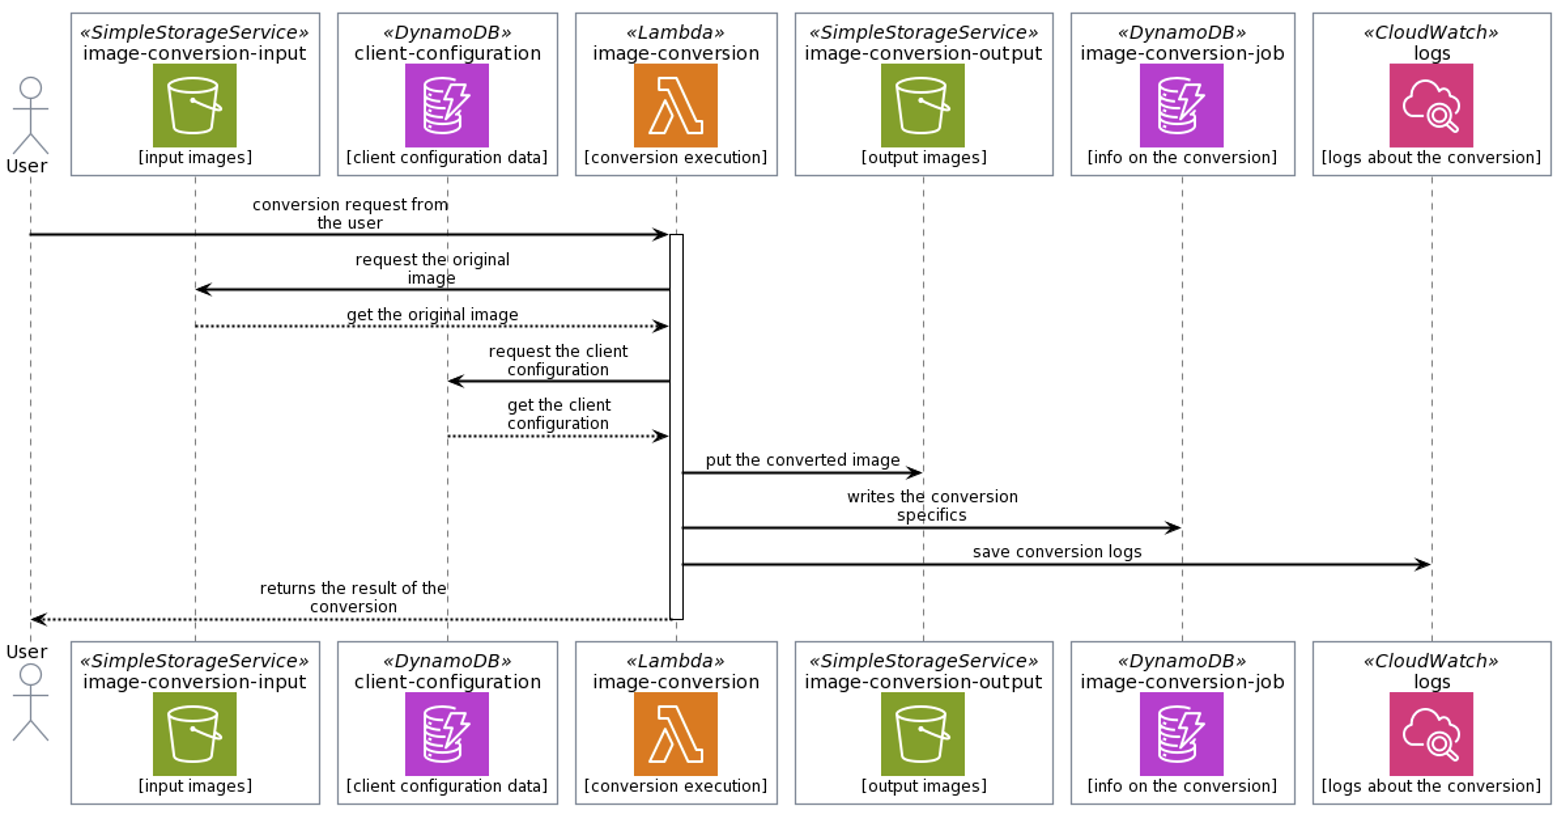
\includegraphics[width=1\textwidth]{images/diagramma-flusso.png}
      \caption{Diagramma di flusso del sistema}
      \label{fig:diagramma-flusso}
\end{figure}

\subsection{Confronto con l'architettura precedente}

Essendo il progetto di stage destinato alla sostituzione di un servizio
attualmente in produzione, è stato necessario confrontare l'architettura
esistente con quella proposta. Le principali differenze sono le seguenti:
\begin{itemize}
      \item \textbf{\emph{deprecazione delle step-function:}} il servizio attuale
            prevede l'utilizzo di \emph{AWS Step Functions}, un servizio che si occupa
            di orchestrare i servizi ad esso legati. L'implementazione di questo
            servizio viene realizzata tramite una macchina a stati, che gestisce il
            flusso di esecuzione in base agli eventi ricevuti. Tra gli eventi
            ricevuti si evidenzia la presenza di una chiamata che permette di
            pulire dall' \glsfirstoccur\gls{EFS} (\emph{Elastic File System}) le
            immagini convertite. \\
            Nel progetto di stage è stato deciso di rimuovere l'utilizzo delle
            \emph{step-functions} per semplificare il flusso della conversione e
            rendere il sistema più semplice da mantenere e da migliorare;
      \item \textbf{\emph{deprecazione dell'EFS:}} il servizio attuale prevede
            l'utilizzo di \emph{EFS} per gestire le immagini da convertire e le
            immagini convertite. \\
            Nel progetto di stage è stato deciso di rimuovere l'utilizzo di \emph{EFS}, in
            quanto la responsabilità della gestione dell'immagine in ambiente
            \emph{serverless} viene delegata completamente al processo eseguito
            dalla \emph{Lambda}, ed eventuali file temporanei non devono più
            essere gestiti manualmente.
\end{itemize}

Queste scelte architetturali portano tuttavia ad una limitazione rispetto al servizio
attualmente in uso, ovvero l'impossibilità di assegnare manualmente la memoria
\emph{RAM} al servizio di conversione. Questa limitazione è dovuta al fatto che
la funzione \emph{Lambda} ha una capacità di memoria massima pari a $10240$
\emph{MB}, impedendo l'eventuale conversione di immagini con un peso
superiore.\\
Questa è considerata una limitazione facilmente superabile per due motivi:
\begin{itemize}
      \item il limite di memoria utilizzabile dalla funzione \emph{Lambda} può essere
            contrattato con \emph{AWS}, nel caso vi fosse la necessità di gestire immagini
            con peso superiore al limite attuale;
      \item secondo una analisi delle conversioni effettuate dal servizio attuale,
            prendendo in considerazione tutte le immagini caricate nella piattaforma
            durante il mese di settembre 2023, è stato identificato che il peso medio di
            un'immagine equivale a $9.02$ \emph{MB}, con un peso massimo raggiunto di $2.03$
            \emph{GB}: entrambe le dimensioni sono ampiamente al di sotto della quota di
            memoria prevista per la funzione \emph{Lambda}.
\end{itemize}


